\subsection{Outline how spontaneous emission can be included in the semiclassical description of atom-light interaction and discuss the result using the optical Bloch vector.}


I den semiklassiske beskrivelse af atom-lysinteraktion ser man lyset som værende en elektromagnetisk bølge, som beskrives klassisk, og ser atomet, som værende et toniveausystem, som er beskrevet kvantemekanisk, og man gør brug af dipolapproksimationen\footnote{Dipolapproksimationen holder så længe, at lysets bølgelængde er større end atomet, $\lambda \gg a_0$.}. Lysbølgen perturberer systemet således, at det vil begynde at oscillere mellem grundtilstanden og den exciterede tilstand, hvilket hedder \textsf{Rabioscillationer}, og disse opstår kun, når der ikke er spontan emission. Disse oscillationer kan beskrives ved Blochligningerne
\begin{align}
    \Dot{\Vec{R}} &=
        \begin{pmatrix}
            \Dot{u} \\
            \Dot{v} \\
            \Dot{w}
        \end{pmatrix}
    =
        \begin{pmatrix}
            \delta v \\
            -\delta u + \Omega w \\
            -\Omega v
        \end{pmatrix}
    = \Vec{R} \cross \left(\Omega\Hat{e}_1 + \delta\Hat{e}_3\right)
    = \Vec{R} \cross \Vec{W} \: ,
\end{align}
hvor $\delta = \omega - \omega_0$ er detuningen\footnote{Dette er en fordanskning af ''the detuning'' på engelsk.} mellem lysets frekvens og atomets resonansfrekvens, $\Omega$ er Rabifrekvensen, som driver overgange mellem de to niveauer i atomet, og $w = \rho_{11} - \rho_{22}$ er forskellen i populationen af de to niveuer.

Problemet ved denne beskrivelse er, at den ikke tager højde for spontan emission, men kun arbejder med absorption og stimuleret emission.


\paragraph{Dæmpning af en klassisk dipol:} Man kan se Rabioscillationerne som værende dreven harmonisk oscillator, hvortil man tilføjer en dæmpning, nemlig den spontane emission. Ved at betragte analogien til den klassiske dipol retfærdiggøres det, at der skal inkluderes et dæmpningsled i de optiske Blochligninger for at medtage spontan emission.

Benyttes Newtons anden lov for en harmonisk oscillator med naturlig vinkelfrekvens $\omega_0$ fås følgende bevægelsesligning
\begin{align} \label{eq:Q18_EquationOfMotionDampedHarmonicOscillator}
    \Ddot{x} + \beta \Dot{x} + \omega_0^2 x &= \frac{F(t)}{m}\cos(\omega t) \: ,
\end{align}
hvor drivkraften har amplituden $F(t)$, som ændres meget langsomt sammenlignet med oscillationen grundet drivfrekvensen, og dæmpningen er $\beta = \alpha/m$, hvor friktionskraften er givet ved $F_\text{friction} = -\alpha\Dot{x}$ og $m$ er massen.

Som løsning til \cref{eq:Q18_EquationOfMotionDampedHarmonicOscillator} ledes efter en løsning på formen
\begin{align} \label{eq:Q18_FormOfTheSolution}
    x &= \mathcal{U}(t)\cos(\omega t) - \mathcal{V}(t)\sin(\omega t) \: ,
\end{align}
hvor første led er den del af forskydningen (eng. the displacement), som er i fase med kraften, mens andet led er faseforskudt foran\footnote{A phase lead occours when $\mathcal{V}(t) > 0$, since $-\sin(\omega t) = \cos(\omega t + \pi/2)$, and $\mathcal{V}(t) < 0$ corresponds to a phase lag.} (eng. phase lead) på $\pi/2$ med hensyn til $F\cos(\omega t)$. \Cref{eq:Q18_FormOfTheSolution} forventer, at det meste af tidsafhængigheden af løsningen giver en oscillation med frekvens $\omega$. Benyttes denne løsning i \cref{eq:Q18_EquationOfMotionDampedHarmonicOscillator}, hvorefter ledene med trigonometriske funktioner forsvinder ved at ''equating the terms that depend on $\sin(\omega t)$ and $\cos(\omega t)$'', hvilket giver
\begin{align}
    \Dot{\mathcal{U}} &= (\omega - \omega_0)\mathcal{V} - \frac{\beta}{2}\mathcal{U} \: , \label{eq:Q18_DotU} \\
    \Dot{\mathcal{V}} &= -(\omega - \omega_0)\mathcal{U} - \frac{\beta}{2}\mathcal{V} - \frac{F(t)}{2m\omega} \: . \label{eq:Q18_DotV}
\end{align}
Amplituderne $\mathcal{U}$ og $\mathcal{V}$ ændrer sig med tiden som amplituden af kraften ændres, idet at vi har antaget, at kraften ændrer sig meget langsomt sammenlignet med oscillationen grundet drivfrekvensen, så må dette også gøre sig gældende for $\mathcal{U}$ og $\mathcal{V}$. Dette kaldes den \textsf{langsomtændrende konvolut-approksimation} (eng. slowly-varying envelope approximation), hvilken er blevet brugt til at udlede \cref{eq:Q18_DotU,eq:Q18_DotV}. Denne approksimation går ud på, at $\Ddot{\mathcal{U}}$ og $\Ddot{\mathcal{V}}$ er blevet negligeret\footnote{Da $\Ddot{\mathcal{U}} \sim \Ddot{\mathcal{V}} \ll 1$.}, og $\Dot{\mathcal{V}} \ll \omega \mathcal{V}$.

Den totale energi af systemet er givet som summen af den kinetiske energi ($\frac{1}{2}m\Dot{x}^2$) og den potentielle energi ($\frac{1}{2}m\omega_0^2x^2$), hvorved den totale energi bliver $E = \frac{1}{2}m\omega^2(\mathcal{U}^2 + \mathcal{V}^2)$, idet der gøres brug af approksimationen $\omega_0^2 \simeq \omega^2$, hvilken er gældende, da vi har gjort brug af en antagelse om at $\omega + \omega_0 \simeq 2\omega$ \footnote{Antagelsen er at $\omega^2 - \omega_0^2 = (\omega + \omega_0)(\omega - \omega_0) \simeq 2\omega(\omega - \omega_0)$.}, som kun gør sig gældende, når $\omega$ er tæt på resonansfrekvensen $\omega_0$. Denne energi ændres med raten $\Dot{E} = m_\omega^2(\mathcal{U}\Dot{\mathcal{U}} + \mathcal{V}\Dot{\mathcal{V}})$, og ved brug af \cref{eq:Q18_DotU,eq:Q18_DotV} bliver dette
\begin{align} \label{eq:Q18_DotE}
    \Dot{E} &= -\beta E - F \mathcal{V}\frac{\omega}{2} \: .
\end{align}
Af dette kan det ses, at hvis der ikke er en drivkraft ($F = 0$), så vil energien blot henfalde.


\paragraph{Optiske Blochligninger inkluderende spontan emission:} Et toniveausystem i et atom vil have en energi, som er proportional med populationen i den exciterede tilstand ($\rho_{22}$), $E = \rho_{22}\hbar\omega_0$, så altså $\Dot{E} \propto \Dot{\rho}_{22}$, og vi ved fra vores udregninger af de optiske Blochligninger uden spontan emission, at $\Dot{\rho}_{22} = \Omega v/2$. Sammenlignes dette med \cref{eq:Q18_DotE}, så fås
\begin{align} \label{eq:Q18_DotRho22}
    \Dot{\rho}_{22} &= -\Gamma\rho_{22} + \frac{\Omega}{2}v \: ,
\end{align}
hvor $\Gamma$ er dæmpningsledet. Af \cref{eq:Q18_DotRho22} kan det ses, at uden en Rabifrekvens ($\Omega = 0$), hvilket er drivfrekvensen, så vil populationen i den exciterede tilstand henfalde eksponentielt\footnote{Da $\Dot{x} = -kx \Rightarrow x(t) = x(0)\exp{-\Gamma t}$.}.

Sammenlignes nu $\Dot{\mathcal{U}}$ og $\Dot{\mathcal{V}}$ fra \cref{eq:Q18_DotU,eq:Q18_DotV} med $\Dot{u}$ og $\Dot{v}$ fra de optiske Blochligninger uden spontan emission, så vil de \textsf{optiske Blochligninger} indeholdende spontan emission blive
\begin{align}
    \Dot{u} &= \delta v - \frac{\Gamma}{2}u \: , \label{eq:Q18_DotLilleU} \\
    \Dot{v} &= -\delta u + \Omega w - \frac{\Gamma}{2}v \: , \label{eq:Q18_DotLilleV} \\
    \Dot{w} &= -\Omega v - \Gamma(w - 1) \: , \label{eq:Q18_DotLilleW}
\end{align}
hvilke beskriver excitationen af et toniveausystem grundet interaktion med lys, som har en frekvens tæt på atomets resonansfrekvens, for en overgang, som også kan henfalde ved spontan emission.

Vi betragter nu ligevægtsløsningen\footnote{Ligevægtsløsningen fremkommer idet man indsætter $\Dot{u} = \Dot{v} = \Dot{w} = 0$ ind i \cref{eq:Q18_DotLilleU,eq:Q18_DotLilleV,eq:Q18_DotLilleW} (eng. steady-state solution), hvilket giver tre samtidige løsninger.}, som fremkommer, når vi arbejder med tider, som er meget længere end levetiden for det øvre energiniveau, $t \ll \Gamma^{-1}$,
\begin{align}
    \begin{pmatrix}
        u \\
        v \\
        w
    \end{pmatrix}
    &= \dfrac{1}{\delta^2 + \Omega^2 / 2 + \Gamma^2 / 4}
        \begin{pmatrix}
            \Omega\delta \\
            \Omega\Gamma/2 \\
            \delta^2 + \Gamma^2 / 4
        \end{pmatrix}
        \: .
\end{align}
Disse ligninger viser, at en stærk drivfelt ($\Omega \rightarrow \infty$) vil få populationerne til at fordele sig ligeligt, idet $\rho_{11} - \rho_{22} = w \rightarrow 0$, og dette kan også ses, hvis vi betrager den exciterede population direkte
\begin{align}
    \rho_{22} &= \frac{1 - \omega}{2} = \dfrac{\Omega^2 / 4}{\delta^2 + \Omega^2 / 2 + \Gamma^2 / 4} \rightarrow \frac{1}{2} \: , \quad \text{idet} \quad \Omega \rightarrow \infty \: .
\end{align}


\paragraph{Diskussion af resultatet ved brug af Blochsfæren:} \Cref{eq:Q18_DotLilleU,eq:Q18_DotLilleV,eq:Q18_DotLilleW} kan skrives som $\Dot{\Vec{R}} = \Vec{R} \cross \Vec{W} - \Gamma \Vec{A}$, hvor $\Vec{A} = (u/2,\: v/2,\: w - 1)$. Blochvektoren $\Vec{R}$ forbliver altså den samme, mens de optiske Blochligninger blot tilføjes et dæmpningsled. Grundet dæmpningsledet, så vil Blochsfæren dog over tid blive mindre og mindre, da $\Vec{A}$'s første- og andekomponenter er parallelle med $\Vec{R}$'s, men dog af den halve længde.

\begin{figure}[!h]
    \centering
    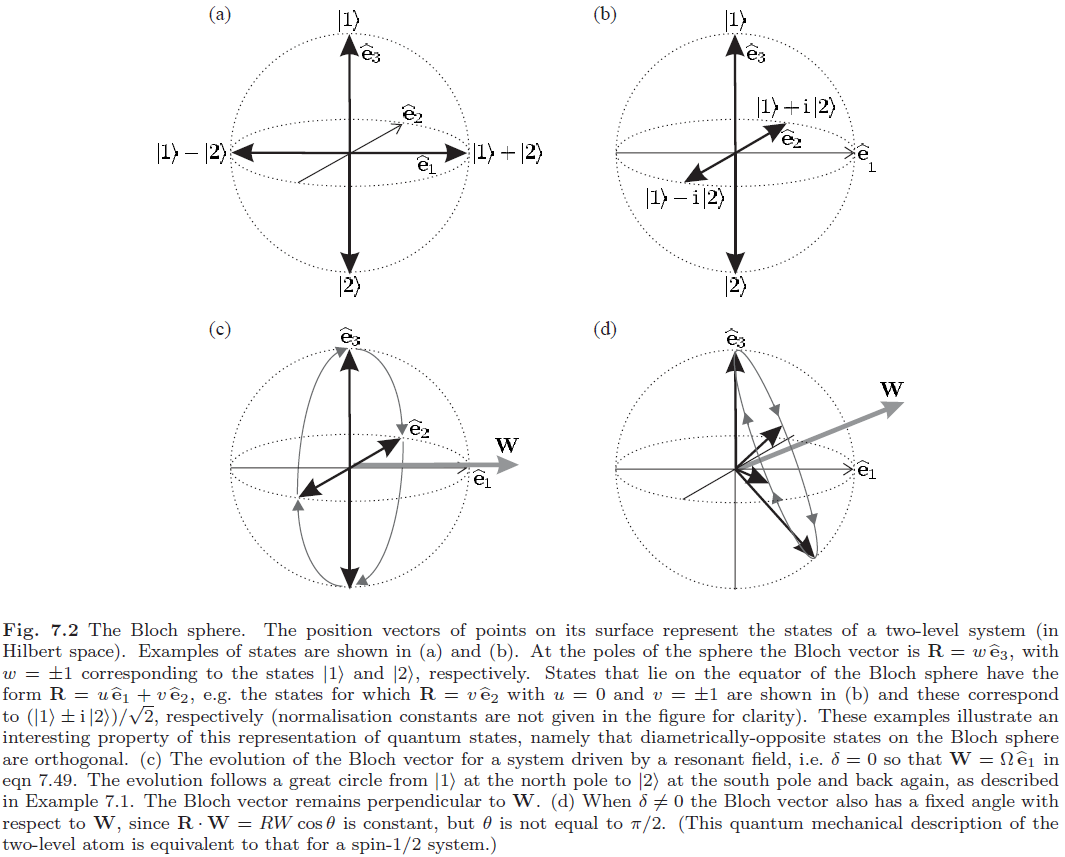
\includegraphics[width=\textwidth]{Q18/images/BlochSphere.PNG}
    \caption{}
    \label{fig:Q18_BlochSphere}
\end{figure}